% Second half of the results section and the discussion (included by main.tex).

\subsection{Sensitivity to the parameters $k$ and $t$}
The parameters are prescribed for asymptotic reasons, and both papers leave their constants open. Fig.~\ref{fig:params} shows the running time on SF for all combinations of $k\in\{1,\dots,6\}$ and $t\in\{2,\dots,10\}$, with the number of levels following from $t$. Three observations hold on both SF and NA. First, $k=1$ is uniformly poor: without frontier reduction every frontier vertex goes through the recursion, and on SF the algorithms are up to \ParSFTwoFiveWorst{} (\bmA) and \ParSFTwoSixWorst{} (\bmB) times slower than Dijkstra. Second, the prescribed values are good but not the best. For \bmA{} a larger $k$ helps, which is consistent with the structure of these networks: with an average degree between 2.0 and 2.6 they consist largely of chains, and more relaxation rounds complete longer chains inside \fp. The fastest setting on SF is $k=\ParSFTwoFiveBestK$, $t=\ParSFTwoFiveBestT$ (\ParSFTwoFiveGain\% faster than prescribed) and on NA $k=\ParNATwoFiveBestK$, $t=\ParNATwoFiveBestT$ (\ParNATwoFiveGain\% faster). For \bmB{} the fastest settings use $t=\ParSFTwoSixBestT$ on both networks, which gives two levels instead of four, and are \ParSFTwoSixGain\% (SF) and \ParNATwoSixGain\% (NA) faster. Third, no setting changes the conclusion: the best ratios to Dijkstra over the whole grid are \ParSFTwoFiveBest{} and \ParSFTwoSixBest{} on SF and \ParNATwoFiveBest{} and \ParNATwoSixBest{} on NA.

\begin{figure*}[t]
\centering
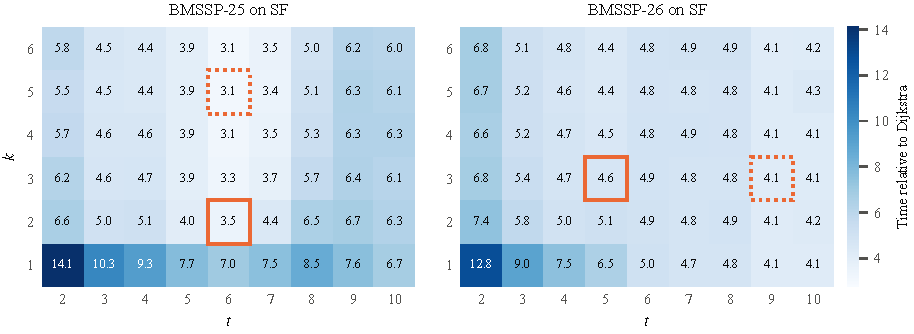
\includegraphics[width=\textwidth]{params_heatmap}
\caption{Running time relative to Dijkstra on SF for every combination of $k$ and $t$ (lighter is faster). Solid box: parameters prescribed by the respective paper; dotted box: fastest combination.}
\label{fig:params}
\end{figure*}

The topmost level of \bmB{} deserves a remark. The call one level below the top may complete up to $t^32^{(L-1)t}$ vertices, where $L=\lceil\log n/t\rceil$, and this is at least $n$ whenever $t^3\ge 2^t$, that is, for $t\le 9$. For every $n$ up to $2^{40}$ (Table~\ref{tab:params}) the top call therefore pulls the source, receives all of $V$ from its single sub-call and relaxes every arc once more without effect. This is visible in the counts: \bmB{} scans every arc once in a base case and once per level.

\subsection{Scaling on synthetic families}
Fig.~\ref{fig:scaling} shows the time relative to Dijkstra as $n$ grows from $2^{10}$ to $2^{\ScaleRandMaxExp}$ (random and grid) or $2^{\ScaleBaMaxExp}$ (preferential attachment and hub). On random digraphs the ratio falls steadily, from \ScaleRandTwoFiveFirst{} at $n=2^{10}$ to \ScaleRandTwoFiveLast{} at $n=2^{22}$ for \bmA{} and from \ScaleRandTwoSixFirst{} to \ScaleRandTwoSixLast{} for \bmB. Preferential-attachment graphs behave alike (\ScaleBaTwoFiveLast{} and \ScaleBaTwoSixLast{} at $n=2^{21}$); the heavy-tailed degree distribution makes no visible difference. On grids the improvement stops early: from $n=2^{14}$ on both algorithms stay between \GridLateMin{} and \GridLateMax{} times slower than Dijkstra. On hub graphs \bmA{} improves to \ScaleHubTwoFiveLast{} while \bmB{} is still \ScaleHubTwoSixLast{} times slower at the largest size. \bmB{} was the slower of the two new algorithms on all \SynthPoints{} synthetic instances, and neither overtakes Dijkstra anywhere in the tested range. The curves are not smooth because the prescribed $k$, $t$ and number of levels are rounded and change in steps. Above $2^{20}$ vertices the two Dijkstra variants themselves separate, the \textsc{DecreaseKey} variant becoming up to \DkLargeMax{} times slower, which indicates that at these sizes all algorithms are governed by memory-hierarchy effects that the cost model does not capture.

\begin{figure*}[t]
\centering
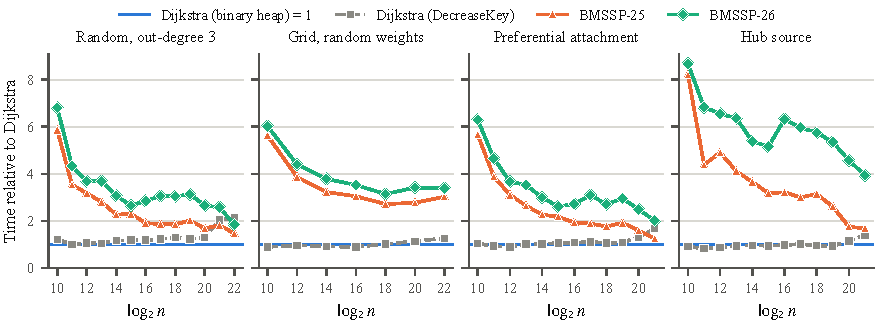
\includegraphics[width=\textwidth]{scaling_ratio}
\caption{Running time relative to Dijkstra with a binary heap on four synthetic families as a function of $n$ (geometric mean over sources).}
\label{fig:scaling}
\end{figure*}

\begin{figure*}[t]
\centering
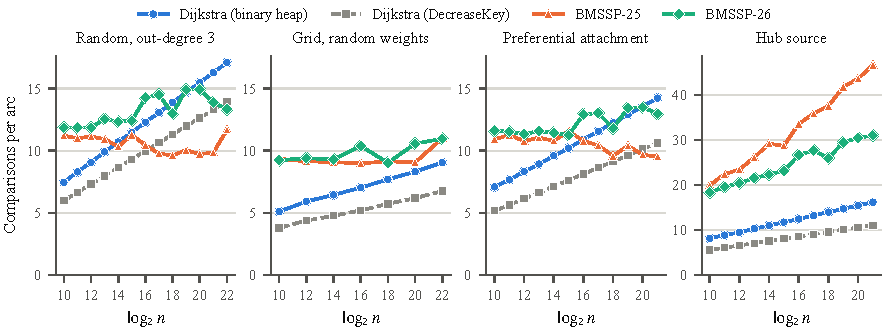
\includegraphics[width=\textwidth]{scaling_cmp}
\caption{Comparisons per arc on the synthetic families as a function of $n$. The hub family has its own vertical scale.}
\label{fig:cmp}
\end{figure*}

Fig.~\ref{fig:cmp} shows the same instances in the cost model of the theorems, and here the picture differs between families. On random and preferential-attachment graphs Dijkstra's comparisons per arc grow linearly in $\log n$, by \SlopeRandDij{} and \SlopeBaDij{} per doubling of $n$ with the lazy heap and by \SlopeRandDijDK{} and \SlopeBaDijDK{} with \textsc{DecreaseKey}. The counts of the BMSSP algorithms are nearly flat, between \CmpRangeRandTwoFiveMin{} and \CmpRangeRandTwoFiveMax{} comparisons per arc for \bmA{} and between \CmpRangeRandTwoSixMin{} and \CmpRangeRandTwoSixMax{} for \bmB{} on random graphs. The curves therefore cross: \bmA{} needs fewer comparisons than binary-heap Dijkstra at every tested size from $n=2^{\CrossCmpRandTwoFiveDij}$ on for random graphs and from $2^{\CrossCmpBaTwoFiveDij}$ on for preferential-attachment graphs ($2^{\CrossCmpRandTwoFiveDijDK}$ and $2^{\CrossCmpBaTwoFiveDijDK}$ against the \textsc{DecreaseKey} variant), and fewer comparisons plus additions from $2^{\CrossOpsRandTwoFiveDij}$ and $2^{\CrossOpsBaTwoFiveDij}$ on. \bmB{} falls below Dijkstra's comparison count at $n=2^{\CrossCmpRandTwoSixDij}$ in both families. This is the asymptotic advantage of the new algorithms appearing at feasible sizes, in the model in which it is proved. It does not carry over to running time: at $n=2^{20}$ on random graphs \bmA{} executes \OpsRandTwentyTwoFive{} comparisons and additions per arc against \OpsRandTwentyDij{} for Dijkstra and still takes \TimeRandTwentyTwoFive{} times as long. On grids and on hub graphs there is no crossing, for two different reasons discussed next.

\subsection{Graph structure: frontier width and maximum degree}\label{sec:structure}
Two properties of the input explain the differences between the families.

\emph{Frontier width.} We measure the width of Dijkstra's frontier by the largest number of vertices its indexed heap holds at any time. On the road networks this is between \RoadPeakMin\% and \RoadPeakMax\% of $n$ (Table~\ref{tab:data}), and on grids it shrinks from \PeakGridSmall\% at $n=2^{10}$ to \PeakGrid\% at $n=2^{22}$. The heap is small, extractions are cheap, and there is little ordering work for a cleverer algorithm to save; Dijkstra's algorithm makes fewer comparisons than both new algorithms at every size. On random and preferential-attachment graphs the frontier holds about \PeakRand\% and \PeakBa\% of the vertices at every size, Dijkstra's algorithm pays the logarithmic factor in full, and the counts of the new algorithms fall below it. Running time orders these inputs the same way: the smallest ratios to Dijkstra occur on random and preferential-attachment graphs, larger ones on grids and road networks.

\emph{Maximum degree.} On hub graphs the frontier is as wide as it can be, since all $n$ vertices are labelled as soon as the source is settled. Nevertheless both BMSSP algorithms need more comparisons than Dijkstra's algorithm, by a factor of \HubCmpRatioMinTwoFive{} to \HubCmpRatioMaxTwoFive{} for \bmA, increasing with $n$, and of \HubCmpRatioMinTwoSix{} to \HubCmpRatioMaxTwoSix{} for \bmB{} (Fig.~\ref{fig:cmp}, right). The counters show why. The $n-1$ arcs of the hub are relaxed together after the first base case. In \bmA{} they all fall into the range that is batch-prepended at level one, where a block holds a single key, so the structure sorts them by repeated median selection; in \bmB{} they are inserted into the search tree of the base case and handed upwards by merges. Either way the algorithm orders the entire frontier, at a higher cost per key than a heap. The analyses exclude this situation by the degree bound, which limits the number of keys one completed vertex can generate. Table~\ref{tab:hub} confirms that the bound is what is missing. After degree reduction with $\delta=3$ the instance has eight times as many vertices and satisfies the precondition, and on it \bmB{} needs fewer than half the comparisons of Dijkstra's algorithm (\HubRedCmpTwoSix{} against \HubRedCmpDij{} per arc of the original graph) and \bmA{} fewer as well (\HubRedCmpTwoFive). The advantage is real but expensive: Dijkstra's algorithm on the original graph needs only \HubCmpDij{} comparisons per arc, the transformation alone makes it \HubRedDijSlow{} times slower, and on the transformed graph \bmA{} and \bmB{} still take \HubRedSameTwoFive{} and \HubRedSameTwoSix{} times as long as Dijkstra's algorithm on the same graph.

\begin{table}[t]
\caption{Hub graph with $n=2^{18}$ as given and after degree reduction. cmp.: comparisons per arc of the original graph; time: relative to Dijkstra on the graph as given}
\label{tab:hub}
\centering
\setlength{\tabcolsep}{3.5pt}
\begin{tabular}{@{}lr|rr|rr|rr@{}}
\hline
 &  & \multicolumn{2}{c|}{Dijkstra} & \multicolumn{2}{c|}{\bmA} & \multicolumn{2}{c}{\bmB}\\
Graph & vertices & cmp. & time & cmp. & time & cmp. & time\\
\hline
\tabinput{tables/hub.tex}
\hline
\end{tabular}
\end{table}

\subsection{Web, road and social graphs}\label{sec:snap}
Table~\ref{tab:snap} repeats the comparison on \SnapGraphs{} larger real graphs. Dijkstra's algorithm is the fastest on all \SnapInstances{} instances: \bmA{} is between \SnapRatioMinTwoFive{} and \SnapRatioMaxTwoFive{} and \bmB{} between \SnapRatioMinTwoSix{} and \SnapRatioMaxTwoSix{} times slower, and \bmB{} is the faster of the two on \SnapTwoSixFaster{} of them. The closest result is \SnapBestInstance, the densest graph with the widest frontier. With unit weights, the setting in which~\cite{ryu2025} reports its simplified solver ahead of Dijkstra, the published algorithms are \SnapUnitTimeMinTwoFive{} to \SnapUnitTimeMaxTwoFive{} (\bmA) and \SnapUnitTimeMinTwoSix{} to \SnapUnitTimeMaxTwoSix{} (\bmB) times slower; we observe no advantage on any graph.

The counts follow the pattern of Section~\ref{sec:structure}. The three road networks have frontiers of at most \SnapRoadPeakMax\% of $n$, and both new algorithms need more comparisons than Dijkstra's algorithm with either weighting. The web and social graphs have frontiers between \SnapOtherPeakMin\% and \SnapOtherPeakMax\% of $n$; with random weights \bmA{} needs fewer comparisons than the lazy-heap baseline on \SnapFewerCmpTwoFive{} of them (\SnapFewerListTwoFive), the two largest. Two qualifications apply. Measured against the \textsc{DecreaseKey} variant, whose heap never holds more than $n$ entries and is therefore much cheaper on dense graphs, \bmA{} needs fewer comparisons on \SnapFewerCmpDKTwoFive{} of the \SnapInstances{} instances. And with unit weights, where Dijkstra's algorithm needs few comparisons per arc, the new algorithms need more on every graph (\SnapUnitCmpMinTwoFive{} to \SnapUnitCmpMaxTwoFive{} times for \bmA).

\begin{table}[t]
\caption{SNAP graphs. Front.: peak frontier of Dijkstra in percent of $n$ (random weights). For each of the two new algorithms: running time relative to Dijkstra with unit weights (unit) and with random weights (rand.), and comparisons relative to Dijkstra with random weights (cmp.)}
\label{tab:snap}
\centering
\setlength{\tabcolsep}{2.6pt}
\begin{tabular}{@{}lrrr|rrr|rrr@{}}
\hline
 & $n$ & $m$ & front. & \multicolumn{3}{c|}{\bmA} & \multicolumn{3}{c}{\bmB}\\
 & ($10^3$) & ($10^6$) & (\%) & unit & rand. & cmp. & unit & rand. & cmp.\\
\hline
\tabinput{tables/snap.tex}
\hline
\end{tabular}
\end{table}

\subsection{Density and weight range}
Two sweeps on random digraphs with $n=2^{18}$ vary further properties. Increasing the average out-degree from 2 to 8 lowers the ratio to Dijkstra from \DensLowTwoFive{} to \DensMinTwoFive{} for \bmA{} and from \DensLowTwoSix{} to \DensMinTwoSix{} for \bmB; beyond that the ratio stays roughly constant. Denser graphs spend a larger share of the time in plain edge scans, which all algorithms perform, but the BMSSP algorithms scan each arc three to four times, so the ratio does not approach one. The weight range has little influence: from unit weights, where all paths with the same number of arcs tie and the tie-breaking rule decides many comparisons, to weights up to $2^{30}$ the ratio stays between \WeightMinTwoFive{} and \WeightMaxTwoFive{} for \bmA{} and between \WeightMinTwoSix{} and \WeightMaxTwoSix{} for \bmB.

\subsection{Memory}
The BMSSP implementations keep one direct-address table per recursion level in addition to the labels. On the random graph with $n=2^{22}$ the peak resident set of the whole process, which includes the graph and the reference solution, is \MemDij~MB for Dijkstra, \MemTwoFive~MB for \bmA{} and \MemTwoSix~MB for \bmB, a factor of \MemRatioTwoFive{} and \MemRatioTwoSix.

\section{Discussion}\label{sec:discussion}
\emph{What \bmB{} gains over \bmA.} The redesigned \fp{} does what it promises. On the road networks it accounts for \PivotScanMinTwoSix{} to \PivotScanMaxTwoSix{} edge scans per arc, against \PivotScanMinTwoFive{} to \PivotScanMaxTwoFive{} for the relaxation rounds of \bmA. The saving is consumed by side effects of the new parameter setting. The value of $t$ is smaller than in \bmA{} (Table~\ref{tab:params}), which gives more levels, and every level relaxes all arcs once: the relaxation loops cost \MainScanMinTwoSix{} to \MainScanMaxTwoSix{} scans per arc against \MainScanMinTwoFive{} to \MainScanMaxTwoFive. In addition the base case is now a search-tree Dijkstra over up to $t^3+1$ vertices instead of a heap with a handful of entries. In total \bmB{} performs more additions than \bmA{} on \RoadsMoreAddsTwoSix{} of the five road networks and more comparisons on \RoadsMoreCmpTwoSix{} of them, and it was slower on \RealTwoSixSlowerWord{} of the five road networks and on all synthetic instances. When $t$ is chosen freely the fastest configurations of \bmB{} have two levels (Fig.~\ref{fig:params}), which suggests that the balance between $t$ and the cost of \fp{} that is optimal asymptotically is not the practical one at these sizes.

\emph{Where the time goes.} On narrow-frontier inputs the new algorithms lose twice: they execute \OpsRatioMinTwoFive{} to \OpsRatioMaxTwoFive{} (\bmA) and \OpsRatioMinTwoSix{} to \OpsRatioMaxTwoSix{} (\bmB) times as many comparisons and additions as Dijkstra's algorithm on the road networks, and each counted operation costs them \PerOpMinTwoFive{} to \PerOpMaxTwoFive{} and \PerOpMinTwoSix{} to \PerOpMaxTwoSix{} times as much time. On wide-frontier inputs of bounded degree the first handicap disappears as $n$ grows, but the second remains and by itself keeps the new algorithms behind. It is tied to features of the design that the cost model does not penalize: every arc is scanned three to five times instead of once, labels are four-field tuples instead of single numbers, and the block structures add indirection and bookkeeping. Reducing the number of passes over the arcs, for instance by skipping the redundant topmost level of \bmB, attacks the right term, but our parameter sweep indicates gains of tens of percent, not factors.

\emph{Relation to earlier measurements.} Our conclusion agrees with every study of an implementation that follows the published algorithm: \cite{castro2025} report Dijkstra to be three to four times faster on large instances, \cite{valko2025} find it faster on Lightning Network graphs, and the solver of~\cite{ryu2025} that follows the paper is reported as two to four times slower. Since our \bmA{} has the same structure as the worst-case implementation of~\cite{castro2025} (the same parameters, per-level tables and deletion repair), their published numbers also serve as a check that our implementation is not unduly slow. On random graphs with $m=3n$ they report 10.7~ms for Dijkstra and 38.2~ms for BMSSP at $n=2^{16}$, 421 and 1286~ms at $2^{20}$, and 2023 and 7703~ms at $2^{22}$ on an Intel i5-10400F; we measure \MsSixteenDij{} and \MsSixteenTwoFive~ms, \MsTwentyDij{} and \MsTwentyTwoFive~ms, and \MsTwentyTwoDij{} and \MsTwentyTwoTwoFive~ms on an Apple M1. Both of our programs are faster in absolute terms, the BMSSP implementation by the larger margin, so our ratios (\RatioRandSixteenTwoFive, \RatioRandTwentyTwoFive{} and \RatioRandTwentyTwoTwoFive) are lower than theirs (3.6, 3.1 and 3.8). The two series also differ in shape: their ratio falls from 25 at $n=2^{7}$ to about three at $2^{14}$ and then stays between 2.8 and 3.8 up to $2^{25}$, whereas ours keeps declining slowly up to $2^{22}$. The machines and graph generators differ and we did not run their code, so we cannot say whether this reflects the implementations or the hardware, and the comparison is indicative only. The reports of a practical advantage over Dijkstra that we are aware of~\cite{ryu2025,webb2025} concern simplified variants on unit-weight graphs (Section~II), and Section~\ref{sec:snap} shows no such advantage for the published algorithms on the same graphs.

\emph{Threats to validity.} All timings come from one machine and one compiler. The implementations follow the pseudocode and use sensible engineering (flat arrays, direct-address tables, no per-call allocation), but they are not tuned to the limit, and the base case of \bmB{} uses a node-based search tree because its pseudocode asks for one. The operation counts are independent of these choices only in part: they depend on the heap and selection routines used, and a heap with fewer comparisons per operation would shift Dijkstra's curves downward. Weights are integers; rounding effects of floating-point weights were not studied. The largest instances have $2^{22}$ vertices, which is far from the regime in which the asymptotic bounds separate, and we make no claim about where a crossover in running time would occur. Finally, the two observations of Section~\ref{sec:correct} concern our reading of the pseudocode of~\cite{duan2026} and have not been confirmed by its authors.
